%=========================================================================
% (c) Michal Bidlo, Bohuslav Křena, 2008

\newtheorem{definice}{Definice}

\chapter{Úvod}\label{uvod}
	Výškoměr je jedním z nepostradatelných přístrojů pro navigaci za letu. Je důležité aby fungoval správně ve~všech situacích, jelikož~chyba v~měření může znamenat havárii letadla. V~lepším případě dojde "pouze" ke~škodám na~majetku, v~horším případě může dojít i~ke~ztrátám na~životech. Plní nezastupitelnou úlohu, díky níž mohou piloti bezpečně létat i~za~špatné viditelnosti.
	
	\section{Motivace}\label{uvod::motivace}
		Motivace pro tuto práci je zvýšení bezpečnosti a~ulehčení výcviku začínajících pilotů. Jde hlavně o~ulehčení výuky přistání, která začátečníkovi může způsobovat potíže. Jedná se primárně o~výuku dosednutí(anglicky "flare"), kdy musí student stáhnout výkon motoru a~přitáhnutím uvést letoun do~horizontálního letu, ideálně několik centimetrů nad dráhou. Student pomalu přitahuje knipl, tímto~zvyšuje úhel náběhu a~letadlo postupně zpomaluje. V~okamžiku, kdy je úhel náběhu příliš velký a~rychlost letadla moc nízká, křídla ztratí vztlak a~letadlo dosedne na dráhu. Pokud student udržuje letadlo v~horizontálním letu nad dráhou ve~velké výšce, může být dosednutí tvrdší, než na~které~je stavěn podvozek, a~může dojít k~poškození podvozku či~zranění posádky i~cestujících.
	
	\section{Cíle}\label{uvod::cile}
	Cílem této práce není, jak se může zdát, zpracování signálů. Prvním cílem této práce je úvod historie vývoje avioniky, hlavně výškoměrů. Druhým cílem je úvod do problematiky měření výšky již od jejího počátku. Dále bude čtenář stručně seznámen s~vývojem radarů, dozví se, jak se radary dělí a~k čemu se jednotlivé typy využívají.
	Třetím cílem je popis problému výuky přistání a~důvod pro zadání této práce, jakožto i~jejího řešení. Dalším cílem je návrh takového systému, který~splní veškeré požadavky na bezpečnost letového provozu na letištích, zvýší bezpečnost výuky přistání a~samozřejmě zjednoduší samotnou výuku. V ideálním případě dojde i~k implementaci a~vzniku samotného systému, jeho integrace do letadla a~úspěšnému otestování.


\chapter{Historie}
	\section{Vývoj přístrojů}
	
		V roce 1903 bratři Wrightové uskutečnili první řízený motorový let. Trval jen chvíli, ale~byl to~přelom v~technologii dopravy. Tímto začala éra letectví. Za první světové války, kdy došlo k~prvnímu masivnímu rozšíření letadel,  ať~již k~průzkumným účelům, bombardování nebo~vzdušným soubojům byli piloti omezeni počasím a~za špatného počasí nemohli létat, jelikož neexistovala technologie, která by umožnila pilotovi nespoléhat pouze na svůj zrak a~navigovat za letu i~jinak, než~pouze vizuálně. Toto vedlo ke~snahám vyvinout systém, který~by~umožňoval navigaci za~jakýchkoliv podmínek. Za~jasného slunečného počasí nebo třeba v~bouřce.\par
		
		Začaly se objevovat první přístrojové desky a~na nich první přístroje. Kvůli omezené ploše palubní desky se na ni moc přístrojů nevlezlo, proto na ni bylo umístěno pouze několik nejdůležitějších přístrojů. Mezi tyto přístroje patřil kompas, teploměr oleje, otáčkoměr, ukazatel indikované rychlosti a~samozřejmě výškoměr. S tímto primitivním vybavením se museli spokojit piloti během první světové války i~v období míru po ní. Postupem času toto omezené vybavení přestalo splňovat podmínky pro přístrojové lety a~s nástupem nových technologií se na palubní desku muselo vejít mnohem více zařízení. Každé letectvo prodělalo vývoj, bohužel, nejrychlejší byl v~dobách druhé světové války, kdy došlo k nejrychlejšímu technologickému pokroku na obou stranách. Rozdíl mezi přístrojovými deskami jednotlivých národů můžeme pozorovat na obrázcích \ref{historie::vyvojPristroju::kokpitG2} a~\ref{historie::vyvojPristroju::kokpitP51}.
		Podoba kokpitu se podstatně neměnila až do příchodu digitální technologie, kdy analogové přístroje nahradily sofistikované systémy zobrazující veškeré údaje potřebné pro všechny fáze letu a~v případě vojenských letounů i~pro bojové situace na displeje v~kokpitu. 
		
		\begin{figure}[H]
			\begin{center}
				\includegraphics[scale=0.42]{obrazky-figures/G2_dashboard.jpg}
				\caption{Přístrojová deska stíhacího letounu Bf109-G2\protect\footnotemark}\label{historie::vyvojPristroju::kokpitG2}
			\end{center}
		\end{figure}
		\footnotetext{zdroj: \url{http://forum.largescaleplanes.com/index.php?showtopic=8725}}
	
		\begin{figure}[H]
			\begin{center}
				\includegraphics[scale=0.4]{obrazky-figures/P51-cockpit-1000.jpg}
				\caption{Kokpit doprovodného stíhacího letounu P51\protect\footnotemark}\label{historie::vyvojPristroju::kokpitP51}
			\end{center}
		\end{figure}
		\footnotetext{zdroj: \url{http://www.warbirdalley.com/p51.htm}}
		
		
	\section{Vývoj měření výšky a~úvod do této problematiky}
	
		Barometry byly lidstvu známy již od~17. století, tyto bohužel obsahovaly vodu. Aby mohl být tlak vzduchu úspěšně změřen, barometr vyžadoval přibližně 10 metrů vysokou trubici. Avšak italskému matematikovi a~fyzikovi Evangelistovi Torricellimu se podařilo zkrátit délku trubice na 80cm nahrazením vody rtutí, která je cca třináctkrát hustší než voda. I přes své relativně malé rozměry je tento barometr pořád příliš velký pro masové rozšíření. Za další zmenšení přístroje je zodpovědný francouzský vědec Lucien Vidi, který vynalezl aneroidní barometr, přezdívaný aneroid\cite{history::aneroid}.\par
		Díky této změně se barometr zmenšil na rozumnou velikost a~již se dal použít v~omezeném prostoru letadel. Ve skutečnosti je barometrický výškoměr pouze překalibrovaný aneroid. Bohužel stejně jako ukazatel indikované rychlosti je závislý na mnoha faktorech. Mimo jiné můžeme jmenovat teplotu a~vlhkost vzduchu. Zásadním problémem je, že~barometrický výškoměr už z principu neukazuje relativní výšku nad terénem, ale~výškud AMSL(height Above Mean Sea Level). Reálně tedy dvě letadla letící podle výškoměru ve výšce 6000 stop několik desítek námořních mil od sebe mohou být v~jiné nadmořské výšce. Na obrázku \ref{historie::vyvojMereniVysky::FL} je názorná ukázka. Zde může čtenáře napadnout, zda se letadla kvůli rozdílným indikovaným hodnotám nesrazí. Barometrické výškoměry sice ukazují nadmořskou výšku špatně, ale~když se letadla přiblíží, tak ukazují stejně špatně a~letadla se tedy minou.\par
		
		\begin{figure}[H]
			\begin{center}
				\includegraphics[scale=0.75]{obrazky-figures/flight_level.png}
				\caption{Rozdíl mezi barometrickou(nadmořskou) výškou a~aktuální výškou}\label{historie::vyvojMereniVysky::FL}
			\end{center}
		\end{figure}
				
		Další potíže nastávají s~rozdílnými atmosférickými tlaky mezi počátečním a~cílovým letištěm. Mějme následující situaci: Letadlo letí z letiště Shiphol v~Amsterdamu, které je tři metry pod hladinou moře, do Himalájí. Zde se v~Tibetu nachází letiště Bangda ve výšce 4334 metrů\cite{bangda}. Rychlou úvahou dojdeme k závěru, že~ si pilot bude muset dávat pozor v~jaké výšce nad terénem letí a~na jakou výšku bude přistávat. Toto bylo vyřešeno přidáním možnosti kalibrace. Pilot před vzletem nastaví hodnotu QNH, kterou pilotovi sdělí řídící letového provozu, taktéž před přistáním učiní řídící v~cílové oblasti. Na obrázku \ref{historie::vyvojMereniVysky::109Altimeter} můžeme vidět bíle okénko ukazující tlak QNH a~kolečno pro jeho nastavení. Do přechodové hladiny se používá tento výškoměr a~nad touto hladinou pilot letí podle druhého výškoměru, který je pevně nastaven na hodnotu 1013.25 hPa. Toto je pevně zavedený standard pro veškeré civilní lety.\par
		
		\begin{figure}[H]
			\begin{center}
				\includegraphics[scale=0.75]{obrazky-figures/109Altimeter.jpg}
				\caption{Výškoměr z letounu Bf109\protect\footnotemark}\label{historie::vyvojMereniVysky::109Altimeter}
			\end{center}
		\end{figure}
		\footnotetext{zdroj: \url{http://www.warbirdsite.com/Collection.html}}
		
		S nástupem satelitních technologií se začaly využívat systémy satelitní navigace. Toto upřesnilo navigaci a~již se nemusíme spoléhat pouze na pozemní kontrolu při určovaní pozice letadla. Pomocí systému GPS je schopna posádka určit přesnou pozici na Zemi, rychlost a~azimut během několika sekund aniž by se musela spoléhat na nepřesné pozemní radary.\par 
		
		\paragraph{Existující radarové výškoměry}
		Dalším zdokonalením bylo uvedení radarových výškoměrů. Ty jsou využívány jako hlavní součást GPWS(Ground Proximity Warning System), kde měří absolutní výšku nad terénem. Toto se využívá ve velkých letadlech vážících desítky tun. Našim cílem je vyvinout dostatečně malý, ale~výkonný vestavěný systém, který by radarové výškoměry zpřístupnil i~pro segment lehkých a~ultralehkých letadel.
	
	\section{Vývoj radaru}
		Zrození radaru se datuje do počátku 20. století, kdy~si mocnosti nezávisle na~sobě uvědomily význam této technologie. Mezi lety 1934 a~1939 začaly USA, Velká Británie, Německo, Sovětský svaz, Japonsko, Nizozemsko, Francie a~Itálie nezávisle na sobě vyvíjet systém detekce pomocí radiových vln.\cite{history::radar} Vývoj radaru výrazně pomohl při~bitvě o~Británii, kdy~britové detekovali formující se letadla Luftwaffe nad Francouzským územím, a~tímto umožnil rychlou odezvu Britských pilotů.\par
			
		Během studené války se radary výrazně zdokonalily. Zvětšil se jejich výkon a~zmenšila se jejich velikost. V současné době se radary houfně využívají k~mírovým účelům, od~sledování počasí přes letectví či~posuny zemské kůry až po mapování.
		
\chapter{Teoretická část}
	
	\section{Radary a~jejich dělení}\label{uvod::radary}
		Radar (\textbf{RA}dio \textbf{D}etection \textbf{A}nd \textbf{R}anging) je systém pro detekci objektů, u kterých~je pomocí rádiových vln schopen určit vzdálenost, azimut a~rychlost sledovaných objektů. Využití radarů je široké, od~mapování terénu, detekce osob přes měření rychlosti vozidel a~využití v~civilním letectví až~po~vojenské účely.	
			
	\paragraph{Klasifikace radarů}
			Radary se dělí podle typu vysílání a~podle použití\cite{radarClasification}. Základní dělení je: 
			\begin{itemize}
				\item \textbf{Primární radar}	-	Slouží k zobrazování objektů ve vzdušném prostoru. Vysílač vysílá vysokofrekvenční signál a~přijímač zachytává ozvěnu vysílaného signálu. Na příslušném místě na obrazovce posléze vykreslí, v~profesním slangu řečeno, knedlík, podle pozice objektu ve vzdušném prostoru vůči radarové stanici.
					
				\item \textbf{Sekundární radar}	-	Slouží k přenosu informací mezi radarovou stanicí a~letadlem. Aby toto spojení fungovalo, musí mít cílový objekt zapnutý transpondér v~příslušném módu, který~po přijetí signálu zpracuje dotaz a~odpoví požadovanými informacemi např. výška, rychlost, souřadnice GPS a~kurz. 
			\end{itemize}
			
			Primární radary se dále dělí na:
			\begin{itemize}
				\item \textbf{Pulsní}	-	Tomuto typu radarů postačuje pouze jedna anténa a~to z~toho důvodu, že~se radar periodicky přepíná mezi vysílacím režimem a~přijímacím režimem. Z tohoto pramení nevýhoda tohoto typu radarů: minimální a~bez modulací i~maximální dosah. Minimální dosah radaru je určen rychlostí přepínaní mezi jednotlivými režimy. Pokud se vrátí ozvěna dříve, než~se radar přepne do~přijímacího režimu, radar objekt nedetekuje a~informace je ztracena. Obdobně to funguje i~u maximálního dosahu. Radar musí zachytit ozvěnu před vysláním dalšího impulsu.
				
				\item \textbf{Kontinuálně vysílající}	-	Radary tohoto typu vysílají nepřerušovaně a~zároveň nepřerušovaně zpracovávají přijatou ozvěnu, proto potřebují jak vysílací, tak přijímací anténu. Tyto radary se dělí na:
					\begin{itemize}
						\item Modulované - Tyto radary využívají frekvenční modulace signálu, díky které jsme schopni vypočítat vzdálenost z~ozvěny vysílaného signálu. Toto je typ radaru, kterým bude vybaveno naše zařízení.
						
						\item Nemodulované - Tyto radary vysílají konstantní signál, který~umožňuje pouze určení rychlosti zachycených objektů. Využívají se k měření rychlosti různých objektů-
					\end{itemize}
			\end{itemize}
		
		\section{Vestavěné systémy}
			Jelikož náš systém má jediný účel, a~to zjistit výšku letadla nad přistávací dráhou, využívat víceúčelová zařízení je pro~nás zbytečně robustní a~neforemné. Potřebujeme jednoduché, rychlé a~elegantní zařízení, které~bude plnit pouze jediný úkol. Zde přicházejí do hry vestavěné systémy.
			
			\begin{definice}
				Vestavěné systémy VS jsou systémy, ve~kterých~je zpracování dat vestavěno/vloženo do~většího systému a~ve~kterém není zpracování dat viditelné uživateli prostřednictvím např. PC počítače. Anglicky se vestavěné systémy označují jako \textbf{embedded system}\cite{impSkripta}.
			\end{definice}
			
			Vestavěné zařízení je jednoduchý a~elegantní způsob řešení jednotvárných algoritmických úloh. Naše úloha musí být vykonávána v~reálném čase, tzn. máme určenou dobu odezvy a~tu musíme splnit. Nutnost mít co nejnižší odezvu určuje nároky na~zvolené zařízení. Na tomto zařízení poběží pouze jediná aplikace. To nám umožňuje optimalizovat aplikaci na~míru systému pro dosažení co~největšího výkonu.
			Bohužel optimalizace aplikace není vše. Aby se algoritmus vykonával co~nejrychleji, musíme pro ni~zvolit odpovídající zařízení. Pro náš systém potřebujeme zajistit dostatečně rychlé vzorkování abychom zabránili aliasingu. Toto je nejlepší řešit na~hardwaru, jelikož rychlost zpracování bude vyšší a~budeme schopni zaručit splnění podmínky Nyquistova teorému, kdy~vzorkovací frekvence musí být alespoň dvakrát větší než~maximální frekvence signálu: \[f_v > 2f_{max}\]
			
			Pro tuto úlohu se hodí programovatelné hradlové pole FPGA. Toto pole bude vzorkovat signál s~dostatečnou frekvencí a~po sběrnici jednotlivé vzorky posílat dále do procesoru pro zpracování.\par
			
			\paragraph{Xilinx Zynq}
				Po určení požadavků na~hardware v~úvahu připadají zařízení od~výrobce programovatelných hradlových polí Xilinx. Konkrétně rodina procesorů Zynq, která~kombinuje FPGA s~procesorovým jádrem ARM Cortex.
				Jak již bylo zníněno výše, FPGA navzorkuje signál a~pošle jej k~dalšímu zpracování přez AXI porty jádru procesoru ARM, na kterém poběží odlehčená verze Linuxu. Na tomto operačním systému poběží aplikace provádějící potřebné výpočty a~bude posílat výsledek na výstup.
				
				\begin{figure}[h]
					\begin{center}
						\includegraphics[scale=0.6]{obrazky-figures/zynq-mp-core-single.png}
						\caption{Architektura procesoru Zynq-7000\protect\footnotemark}
						\label{teorie::embedded::zynq}
					\end{center}
				\end{figure}
				\footnotetext{zdroj: \url{https://www.xilinx.com/products/silicon-devices/soc/zynq-7000.html}}
			
			\paragraph{Řídící modul}
				Řídící modul obsahující výše zmíněný procesor je dodán společností CAMEA s.r.o. Modul obsahuje vstupně výstupní porty , které~můžeme využít v~náš prospěch. Jako výstupní porty můžeme využít USB sběrnici s~přímým přístupen do paměti, GPIO porty nebo Serial Peripheral Interface. 
				\begin{itemize}
					\item USB můžeme využít pro přenos přesných informací obrazovou formou na displej, kde zobrazujeme výšku, případně využít externí USB zvukovou kartu pro generování zvukových signálů. 
					
					\item Pomocí GPIO portů, případně rozhraní SPI, můžeme ovládat panel s~LE Diodami, který~barevnými LED seřazenými vertikálně. Tento panel bude mít diody vyzařující světlo od~zeleného spektra, přes žlutou, oranžovou a~sytě červenou, kdy~bude začínat fáze dosednutí.
					
					\item Zvuková komunikace může probíhat generováním tónů a~odesílání konektorem typu 3.5mm Jack. Bude se generovat stále stejný tón konstantní délky, přičemž zkracující se perioda bude signalizovat snižující se výšku. Pokud bude letadlo těsně nad zemí, bude se generovat tón bez přerušení.
				\end{itemize}
			
			\paragraph{Kalibrace modulu}
				Další částí naší úlohy je nutnost kalibrace zařízení, jelikož každé letadlo může mít tento modul umístěno v~jiné výšce nad zemí. Kalibrace může být statická - v~kódu bude přičtena konstanta, nebo dynamická, kdy~se před startem modul zkalibruje. Statická kalibrace má výhodu jednoduššího chování modulu a~bude vyžadovat o~jeden ovládací prvek méně, avšak bude nutno zasahovat do zdrojových kódů při instalaci na jiné letadlo. Dynamická kalibrace, na rozdíl od~statické, má nevýhodu složitějšího řídícího programu, ale~bude možno mít jeden program pro všechny typy letadel. Přidaný ovládací prvek nebude téměř znát. V tomto případě se autor přiklání k~dynamické kalibraci.
				
			\paragraph{Ovládací panel}
				Nutnost kalibrace nás přivádí k~ovládacímu panelu modulu. Přístroj je třeba nějak zapnout, toto bude první přepínač. Dále vyvstává otázka nutnosti mít vždy zapnutou zvukovou signalizaci. Jelikož bude využití tohoto výškoměru při vzletu mizivé, bude dobré, když~bude mít pilot možnost vypnout zvukovou indikaci, která~v~situaci, kdy~ji není potřeba může působit rušivě. Proto může být přítomen přepínač ovládající tuto funkci. Jako třetí kontrolní prvek zvolíme tlačítko spouštějící kalibraci přístroje na referenční hodnotu země. Je nutné, abychom zabránili kalibraci výškoměru ve vzduchu, proto by mělo toto tlačítko být překryté víčkem. V případě, že~bude koncipováno jako ovládací prvek na dotykovém displeji, za~pohybu letadla by mělo být deaktivované.
				
	\section{Fáze přistání}
		Letadlo, které vzlétne, musí zpět na zem. Ideálně rozumným a~hlavně bezpečným způsobem. Není žádoucí, aby se jak letadlu, ale~hlavně pasažérům cokoliv přihodilo. Způsobilo by to nejen finanční ztráty. Proto je kladen velký důraz na výuku a~správné naučení přistávání.  

		\begin{figure}[H]
			\begin{center}
				\includegraphics[scale=0.7]{obrazky-figures/angle_of_attack.png}
				\caption{Proudění vzduchu podél křídla.}
				\label{teorie::pristani::angle_of_attack}
			\end{center}
		\end{figure}
		
		Když se blíže podíváme na přistání, je to doslova řízený pád. Na obrázku \ref{teorie::pristani::angle_of_attack} můžeme vidět příklad proudění vzduchu podél křídla konvenční konstrukce. $F_L$ značí vztlakovou sílu(lift), $F_G$ značí gravitační sílu(gravity), $F_D$ značí odpor vzduchu(drag) a~$\alpha$ značí úhel náběhu. Díky tomuto tvaru nad křídlem proudí vzduch rychleji než pod křídlem, podle Bernoulliho rovnice to znamená, že~nad křídlem má vzduch menší hustotu než pod a~dochází ke vzniku vztlaku. Čím větší je úhel náběhu, tím větší je vztlak a~zároveň se zvětšuje odpor vzduchu. Toto platí pouze za podmínky, kdy je úhel náběhu menší než je jeho kritická hodnota. Od této kritické hodnoty, kterou má každý tvar křídla jinou, dochází ke snižování generovaného vztlaku až k nule ale~odpor vzduchu stále stoupá. To znamená, že~letadlo ztrácí rychlost a~výšku. Na pilotovi je, tento řízený pád udržel v~rozumné míře a~nepropadl se do nekontrolovatelného pádu, jelikož při přistání není mnoho prostoru pro znovuzískání kontroly nad letadlem.\par
		Přistání lze rozdělit do několika fází\cite{landingPhases}.
		
		\begin{enumerate}
			\item STAR(\textbf{S}tandard \textbf{T}erminal \textbf{A}rrival \textbf{R}oute) - Po opuštění letové trasy letadlo provede prvotní přiblížení po trase určené v~letecké informační příručce(AIP). 
			
			\item ILS Přiblížení (\textbf{I}nstrument \textbf{L}anding \textbf{S}ystem \textbf{A}pproach) - Po ukončení STARu pilot na základě uděleného povolení provede přiblížení pomocí přístrojů, které ho přesně navádějí na dráhu. V této fází si pilot připraví letadlo do přistávací konfigurace.
		
			\item Závěrečné přiblížení (Final approach) - Během této fáze pilot musí udržovat přibližovací rychlost danou výrobcem letadla a~letět po kurzu osy dráhy pod sklonem určeným přibližovacími pravidly(glidepath). Zde do hry vstupuje naše zařízení, které bude pilotovi oznamovat výšku stroje nad terénem.
					
			\item Výdrž - Když se pilot přibližuje k~dráze, musí přitáhnout knipl, tím zvýší úhel náběhu a~jak jsme si již vysvětlili výše, způsobí zpomalení stroje. Pilotovým úkolem v~této fázi letu je s~vypnutým motorem udržovat letadlo ve vodorovném letu těsně nad dráhou, na kterou~pak díky ztrátě vztlaku dosedne. Je důležité, aby letadlo bylo těsně nad dráhou, čím výše se v~okamžiku ztráty vztlaku letadlo nachází, tím tvrdší přistání může čekat. A tím větší škody mohou vzniknout.
					
			\item Dosednutí a~rolování (Touchdown and taxi) - Po dosednutí pilot zpomalí letadlo na požadovanou rychlost pro rolování a~roluje na místo určené řídícím letového provozu. 
		\end{enumerate}
				
\chapter{Návrh řešení}\label{navrhReseni}
	Nejdříve si musíme uvědomit, co je našim cílem, analyzovat zadání a~podle něj si pak navrhnout vhodné řešení. Vhodným se rozumí jednoduché, efektivní a~rozšířitelné pro další využití.\par
	
	\begin{figure}[H]
		\begin{center}
			\includegraphics[scale=0.7]{obrazky-figures/navrh_obecne.png}
			\caption{Moduly}
			\label{navrh::moduly}
		\end{center}
	\end{figure}
	
	Kvůli omezenému prostoru naše zařízení byt malé, kvůli zachování aktuálnosti předané informace rychlé, kvůli spotřebě elektrické energie energeticky nenáročné a~kvůli podmínkám, ve kterých bude pracovat odolné vůči vnějším vlivům. Naštěstí nároky na rychlost zpracování nejsou příliš přísné. Průměrný člověk má reakční dobu přibližně sekundu, v~závislosti na tréningu a~požadované reakci. Zároveň ale~platí, že~čím rychlejší náš systém bude, tím přesnější informace budeme schopni dodávat pilotovi. Předané informace musí být ve vhodném formátu pro rychlou a~bezchybnou interpretaci pilotem, aniž by působily rušivě a~odváděly pozornost.
	
	\section{Platforma}\label{navrhReseni::platforma}
		Jak již bylo zmíněno v~úvodu této kapitoly, potřebujeme malé, ale~rychlé zařízení, které bude v~reálném čase poskytovat údaje o~aktuální výšce. V našem případě, vzhledem k~reakční době člověka okolo sekundy, bude stačit, když systém stihne spočítat výsledek a~předat jej pilotovi do $\sim$250ms.\par
		
		Kvůli nárokům na velikost můžeme vyřadit objemné osobní počítače s~architekturou x86 případně AMD64 a~spíše se ponořit do~oblasti vestavěných systémů. V~současnosti trh nabízí dostatečně výkonné a~zároveň dostatečně kompaktní zařízení, která~jsou pro náš účel vhodná. Jako možný kandidát se jeví mikropočítač Raspberry Pi, který už je dostatečně výkonný a~zároveň malý aby mohl splnit požadavky naši úlohu. Bohužel, kvůli konektivitě je tato platforma nevhodná. Jako další se nabízí Arduino. Tato platforma nabízí solidní výkon za rozumné peníze. Bohužel tento výkon nedostačuje našim potřebám a~hodí se spíše do nově rozvíjejícího se oboru Internet of Things. Vhodnější alternativa k~tomuto řešení se jeví procesor rodiny Zynq od~výrobce Xilinx, který je určen přesně pro naše potřeby, a~díky integrovaným programovatelným hradlovým polím FPGA výrazně urychluje zpracování ozvěny signálu byť už jen pouhým vzorkováním daného signálu. Přístroj s~procesorem dodala společnost CAMEA s.r.o. Na tomto procesoru bude spuštěn operační systém OpenSUSE, který bude obsluhovat naši aplikaci.
		
	\section{Radar}
		Radarový transciever, se~kterým~budeme v~této práci pracovat je K-MC1 Radar Transciever firmy RFbeam Microwave GmbH dodaný firmou CAMEA s.r.o. Jedná se o kontinuálně vysílající a~přijímající radar s~frekvenční modulací. Díky frekvenční modulaci vysílaného signálu jsme schopni změřit nejenom rychlost objektu, ale~i~jeho vzdálenost, což je přesně to, co pro naše účely potřebujeme.
	
	\section{Výstupní zařízení}
		Náš systém musí pilotovi nějak interpretovat sesbíraná data, jinak by byl zbytečný. Způsob komunikace musí být tak detailní, aby dokázal předat informace o~výšce nad~zemí a~zároveň dostatečně jednoduchý, aby pilot mohl data ze~systému zpracovat rychle a~efektivně aniž by výstupní zařízení odvádělo pozornost od~právě prováděných úkonů. Jedna z~možností je použití zvukových signálů, druhá je zobrazování aktuálních informací na přístrojové desce letounu. Zde si musíme položit otázku, jaký z těchto způsobů zvolíme. Zobrazení dat na přístrojové desce nabízí možnost jejich nejpřesnější interpretace, bohužel bude odvádět pozornost pilota a~zvyšuje se riziko nehody. Jako další nevýhodu autor vidí zbytečně zabraný prostor, jehož přidaná hodnota po osazení přístrojem pro zobrazovaní dat není dostatečná pro naše použití. 
			
	\section{Software}\label{navrhReseni::software}
		Zde si musíme připomenout, že~našim úkolem není zpracování signálu. Program pro obsluhu generování informací pro pilota musí být rychlý, spolehlivý a nenáročný.
		
	\section{Komunikační protokol}\label{navrhReseni::protokol}	
	
	\section{Umístění na letadle}\label{navrhReseni::umisteniNaLetadle}
		Zařízení musí být na~letadle umístěno tak, ať~je šance požkození přístroje při tvrdším přistání minimální a~zároveň musí být měření konzistentní. Toto vylučuje umístění přístroje na~konci křídel. Může dojít k~odření křídla o~zem při přílišném naklonění, navíc bude muset být provedena velká korekce výšky a~může dojít k~změnám detekované výšky při náklonech letadla, taky dojde k narušení aerodynamického tvaru křídla. Ideální by bylo umístit senzor na pneumatiky jednoho z~kol hlavního podvozku, bohužel velice rychle zjistíme, že~je to nevhodné řešení z~důvodů jednorázového použití radaru. Jako vhodné možnosti se jeví umístění:
		\begin{itemize}
			\item na~nohu podvozku za předpokladu, že~se na~ni zařízení vejde(v případě zatažitelného podvozku). Při umístění na~pevný podvozek je třeba zamezit možnosti vzniku poškození následkem otřesů při tvrdém přistání. 
			\item na~spodní část kořene křídla, kde~nebude moment síly způsobující rotaci letadla ve~vodorovné ose tak velký, jako na konci křídla. Otřesy, které~bude muset zařízení snášet nebudou tak velké jako na noze hlavního podvozku. Bohužel zde zůstává nutnost korekce podle výšky kořene letadla nad~rovinou podvozku.
			\item na trup letadla, toto bohužel bude vyžadovat vrtání do trupu a~tudíž úpravu konstrukce letadla.
			\item do trupu letadla, ideálně do~odpružené schránky s~dvířky, která by se otevřela při spuštění radaru při náletu na přistání. Opět zde je otázka modifikace konstrukce letadla.
		\end{itemize} 
		Note: Asi bude nejlepší přilepit to na nohu, ať nemusíme vrtat, to je třeba zkonzultovat s~majitelem letadla. Ostaní možnosti jsou příliš drahé.


%=========================================================================
